\documentclass[a4paper,twoside,12pt,openright]{report}

%% Language %%%%%%%%%%%%%%%%%%%%%%%%%%%%%%%%%%%%%%%%%%%%%%%%%
\usepackage[francais]{babel}
\usepackage[utf8]{inputenc}
\usepackage[T1]{fontenc}
\usepackage{lmodern} 
\usepackage{hyperref}

%% Packages for Graphics & Figures %%%%%%%%%%%%%%%%%%%%%%%%%%
\usepackage{graphicx} 

%% Math Packages %%%%%%%%%%%%%%%%%%%%%%%%%%%%%%%%%%%%%%%%%%%%
\usepackage{amsmath}
\usepackage{amsthm}
\usepackage{amsfonts}
\usepackage{fullpage}

\setlength{\parindent}{0cm}
\setlength{\parskip}{1ex plus 0.5ex minus 0.2ex}
\newcommand{\hsp}{\hspace{20pt}}
\newcommand{\HRule}{\rule{\linewidth}{0.5mm}}
%%%%%%%%%%%%%%%%%%%%%%%%%%%%%%%%%%%%%%%%%%%%%%%%%%%%%%%%%%%%%
%% DOCUMENT
%%%%%%%%%%%%%%%%%%%%%%%%%%%%%%%%%%%%%%%%%%%%%%%%%%%%%%%%%%%%%
\begin{document}
\begin{titlepage}
  \begin{sffamily}
  \begin{center}

    \textsc{\LARGE MASTER MIAGE 2ème année \linebreak Université Paris Nanterre}\\[2cm]

    \textsc{\Large Mémoire de fin d’études présenté pour l’obtention du grade de master}\\[1.5cm]

    \HRule \\[0.4cm]
    { \huge \bfseries Comment les flots de contrôle peuvent-ils nous permettre de faire du refactoring de code en Java. \\[0.4cm] }

    \HRule \\[2cm]
    
\includegraphics[scale=0.40]{image/univ.jpg}
    \hspace{2cm}
    
    \vfill
  \begin{minipage}{0.4\textwidth}
      \begin{flushleft} \large
        \textsc{Présenté par :}\\ \textsc{Thibault Sartre}\\
      \end{flushleft}
    \end{minipage}
    \begin{minipage}{0.4\textwidth}
      \begin{flushright} \large
        \textsc{Tuteur :}\\ \textsc{Emmanuel Hyon}\\
      \end{flushright}
    \end{minipage}
    \vfill
    {\large Septembre 2018 — Juillet 2019}
  \end{center}
  \end{sffamily}
\end{titlepage}
\renewcommand{\contentsname}{Sommaire}
\tableofcontents{}
\chapter{Contexte}
\section{Introduction}
Le refactoring est une activité d'ingénierie logiciel consistant à modifier le code source d'une application de manière à améliorer sa qualité sans altérer son comportement vis-à-vis des utilisateurs.
L'objectif du refactoring est de réduire les coûts de maintenance et de pérenniser les investissements tout au long du cycle de vie du logiciel en se concentrant sur la maintenabilité et l'évolutivité.\cite{ref1}\\
"With refactoring you can take a bad design, chaos even, and rework it into well-designed code."\cite{ref2}\\
Le refactoring permet donc de passer d'un code possédant de mauvaise base à un code propre.\\
Un bon refactoring doit pouvoir améliorer la qualité d'un code tout en gardant son fonctionnement du point de vue de l'utilisateur. Concernant la partie des tests, tout les tests qui fonctionnaient avant le refactoring se doivent d'être fonctionnels après.\\
Dans ce mémoire, nous allons analyser différentes techniques de refactoring. Puis nous allons étudier le principe des flots de contrôle.\\ Enfin je vous proposerais et évaluerais une solution pour faire du refactoring de code en utilisant les flots de contrôle pour le langage Java.\\
Ce sujet est intéressant et actuel car il faut commencer à ce soucier du code que l'on produit car plus l'on avance dans le temps plus les programmes sont lourds et contiennent de lignes de code. Avec la puissance des ordinateurs actuels, la plus part des développeurs ne prennent plus le temps d'écrire des codes de qualité car la machine sera de toute façon assez rapide pour compenser un code de mauvaise qualité.\cite{ref4}\\
Avec le temps, la relecture et la modification de code sera difficile avec les programmes qui deviennent de plus en plus gros.\cite{ref4}\\
Pour essayer de diminuer cette quantité de travail à l'avenir, il faut commencer à produire du code de qualité et bien structuré. Concernant les codes déjà existant il faudra donc faire du refactoring de code. Or le refactoring peut-être long selon la qualité des projets que l'on traite. Il serait donc intéressant et très utile d'avoir un programme permettant d'automatiser des parties de refactoring pour permettre de gagner du temps précieux. 
Ce mémoire a pour but de fournir une solution qui permettrais de faire du refactoring de code facilement pour gagner du temps tout en produisant du code de qualité.\cite{ref3}

\chapter{Le refactoring}
\section{Composed Method Pattern}
L'un des grands ennemie des développeurs est de faire des méthodes trop longue qui sont difficilement compréhensible.
Une grande partie du refactoring est donc consacrée à la composition correcte des méthodes.\cite{ref5}\\

L'objectif de cette méthode de refactoring est de :\\
- rendre les méthodes facilement compréhensible.\\
- simplifier les méthodes en les brisants en plusieurs méthodes plus petites.\\
- supprimer la duplication de code.\\
- nommer proprement les variables, méthodes et paramètres pour comprendre leurs utilités au premier coup d'œil.\\
- pouvoir faire des tests plus facilement car les morceaux de méthodes peuvent être testés individuellement.\cite{ref6}\\

\subsection{Extraction de méthode}
\paragraph{Présentation :} 
La technique d'extraction de méthode permet comme son nom l'indique, d'extraire des méthodes (ou fonction) du code. Car plus il y a de ligne dans une méthode plus il est difficile de comprendre ce que fait la méthode.\\
Il faut donc lorsque c'est possible extraire du code pour former d'autre méthode et simplifier le code.
\begin{center}
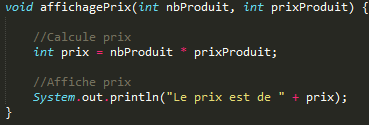
\includegraphics[scale=1]{Image/Extraction_Methode.png}\\
\itshape{Avant extraction de méthode}
\end{center}

\paragraph{Exemple :} 
Au dessus nous avons une méthode qui va afficher le prix d'un produit tout en calculant elle même le prix.\\
Si l'on applique l'extraction de méthode, on va obtenir l'exemple du bas, c'est à dire extraire la méthode de calcule du prix car on en aura surement besoin ailleurs. On remplace donc la calcule du prix dans la méthode affichagePrix par un appel à la méthode calculePrix.\\
\begin{center}
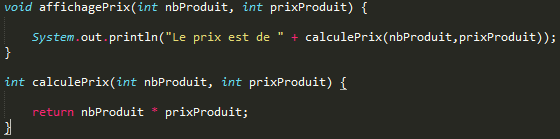
\includegraphics[scale=1]{Image/Extraction_Methode2.png}\\
\itshape{Après extraction de méthode}
\end{center}
\paragraph{Bénéfices :}
Pour que cette technique de refactoring soit la plus efficace, il faut absolument nommer ses méthodes et les paramètres de manière à comprendre très facilement qu'elle est sont but et que représente les paramètres. Le code est donc bien plus lisible.\\\\
A l'aide de cette méthode, on évite la duplication de code. Puisque dans l'exemple on aurait pu vouloir calculer le prix d'un produit dans une autre méthode, avec le code au dessus on aurait dupliqué le code pour calculer le prix d'un produit.\\\\
L'extraction de méthode nous permet aussi d'isoler les parties indépendantes du code. Cela est pratique lorsque l'on cherche un potentiel bug, on peut plus facilement tester toutes les méthodes du codes car elles sont toutes isolées les une des autres.

\paragraph{Technique inverse :}
La technique de refactoring Inline Method est l'exact opposé de l'extraction de méthode. Cette technique consiste à supprimé les méthodes jugées inutile qui sont très courtes ou qui sont plus facilement compréhensible par le code à l'intérieure de la méthode que par son nom. Cela à pour seul but de simplifier le code en diminuant le nombre de méthode dans le code.

\subsection{Extraction de variable}
\paragraph{Présentation :}
La technique d'extraction de variable permet de créer des variables claires qui nous permet de rendre des expressions complexe plus compréhensible.
Elle peut s'appliquer, par exemple, sur les conditions de if ou aussi des expressions arithmétiques sans résultats intermédiaires.

\begin{center}
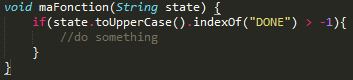
\includegraphics[scale=1]{Image/Extraction_Variable.png}\\
\itshape{Avant extraction de variable}
\end{center}

\paragraph{Exemple :}
Au dessus, nous pouvons voir une fonction qui va faire quelque chose si l'état est done.
Si l'on applique l'extraction de variable, on obtient une variable isDone qui contient un boolean. Cette méthode nous permet de passer d'un code qui contient une expression peu lisible à un code avec une variable explicite.

\begin{center}
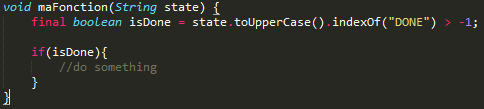
\includegraphics[scale=1]{Image/Extraction_Variable2.png}\\
\itshape{Après extraction de variable}
\end{center}

\paragraph{Bénéfices :}
Pour que le résultat de cette méthode soit optimal, il faut nommer efficacement les variables créées pour  qu'elles soient le plus lisible possible. Cela va permettre de produire un code plus lisible et qui contiendra moins de long commentaire pour expliquer les longues expressions.

\paragraph{Inconvénient :}
Le code va contenir beaucoup de variable mais cela est dérisoire comparé à la lisibilité du code qui est nettement améliorée.

\paragraph{Technique inverse :}
La technique Inline Temp va permettre de supprimer les variables superflue qui contienne uniquement le résultat d'une opération simple qui va être utilisé une seul fois. Cette technique n'a pas de vrai bénéfice dans cette état, en revanche elle peut être couplé avec la technique suivante.

\subsection{Remplacement des temporaires avec des méthodes}
\paragraph{Présentation :}
Le remplacement des temporaires avec des méthodes va comme son nom l'indique, remplacer des variables temporaires par le résultat de méthode. On va extraire le code des variables temporaire avec la technique Inline method puis les placer dans des méthodes.

\begin{center}
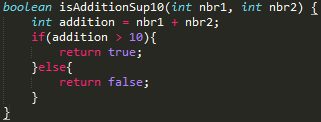
\includegraphics[scale=1]{Image/Remplacement_Temp_Methode.png}\\
\itshape{Avant remplacement du temporaire}
\end{center}

\paragraph{Exemple :}
Au dessus, nous pouvons voir que l'addition des deux paramètre est stocké dans une variable temporaire. Après le refactoring, la variable temporaire disparait et on obtient une méthode qui va s'occuper de faire l'addition à la place.

\begin{center}
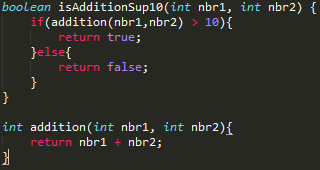
\includegraphics[scale=1]{Image/Remplacement_Temp_Methode2.png}\\
\itshape{Après remplacement du temporaire}
\end{center}

\paragraph{Bénéfices :}
Le code est plus compréhensible grâce au nom de la méthode qui est explicite.\\
Si j'ai besoin plus tard dans mon code de faire une addition, j'ai une méthode que je peux réutiliser.

\subsection{Diviser les variables temporaires}
\paragraph{Présentation :}
Parfois dans nos code, nous déclarons une variable temporaire où nous stockons un résultat quelconque. Puis plus tard, nous réutilisons cette même variable pour stocker un autre résultat n'ayant aucun rapport.
Cette technique a pour but de ne plus utiliser la même variable temporaire pour faire différentes choses.

\begin{center}
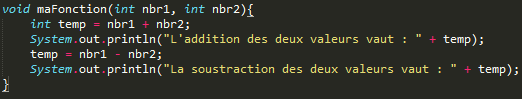
\includegraphics[scale=1]{Image/Diviser_Temp.png}\\
\itshape{Avant division}
\end{center}

\paragraph{Exemple :}
On peut voir au dessus que je réutilise la variable temp pour faire à la fois une addition et une soustraction. Après le refactoring on obtient deux variable proprement nommées addition et soustraction.

\begin{center}
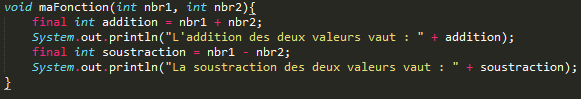
\includegraphics[scale=1]{Image/Diviser_Temp2.png}\\
\itshape{Après division}
\end{center}

\paragraph{Bénéfices :}
Le fait d'avoir chaque variable,méthode ou n'importe quelle composant qui a un unique but permet de faciliter grandement la maintenance du code. Puisque on peut modifier des parties du code sans que ça affecte une autre partie.\\
Cela permet aussi une meilleure relecture du code car on supprime les variables nommées temp ou value pour donner des noms facilement compréhensible.

\subsection{Remove Assignments to Parameters}
s
\subsection{Replace Method with Method Object}
s
\subsection{Substitute Algorithm}
s



\newpage
\section{Déplacement des fonctionnalités entre les objets}
s
\subsection{Move Method}
s
\subsection{Move Field}
s
\subsection{Extract Class}
s
\subsection{Inline Class}
s
\subsection{Hide Delegate}
s
\subsection{Remove Middle Man}
s
\subsection{Introduce Foreign Method}
s
\subsection{Introduce Local Extension}
s



\newpage
\section{Organiser ses données}
s
\subsection{Self Encapsulate Field}
s
\subsection{Replace Data Value with Object}
s
\subsection{Change Value to Reference}
s
\subsection{Change Reference to Value}
s
\subsection{Replace Array with Object}
s
\subsection{Duplicate Observed Data}
s
\subsection{Change Unidirectional Association to Bidirectional}
s
\subsection{Change Bidirectional Association to Unidirectional}
s
\subsection{Replace Magic Number with Symbolic Constant}
s
\subsection{Encapsulate Field}
s
\subsection{Encapsulate Collection}
s
\subsection{Replace Type Code with Class}
s
\subsection{Replace Type Code with Subclasses}
s
\subsection{Replace Type Code with State/Strategy}
s
\subsection{Replace Subclass with Fields}
s



\newpage
\section{Simplifier les expressions de condition}
s
\subsection{Decompose Conditional}
s
\subsection{Consolidate Conditional Expression}
s
\subsection{Consolidate Duplicate and Conditional Fragments}
s
\subsection{Remove Control Flag}
s
\subsection{Replace Nested Conditional with Guard Clauses}
s
\subsection{Replace Conditional with Polymorphism}
s
\subsection{Introduce Null Object}
s
\subsection{Introduce Assertion}
s




\newpage
\section{Simplifier les appels de méthode}
s
\subsection{Rename Method}
s
\subsection{Add Parameter}
s
\subsection{Remove Parameter}
s
\subsection{Separate Query from Modifier}
s
\subsection{Parameterize Method}
s
\subsection{Replace Parameter with Explicit Methods}
s
\subsection{Preserve Whole Object}
s
\subsection{Replace Parameter with Method Call}
s
\subsection{Introduce Parameter Object}
s
\subsection{Remove Setting Method}
s
\subsection{Hide Method}
s
\subsection{Replace Constructor with Factory Method}
s
\subsection{Replace Error Code with Exception}
s
\subsection{Replace Exception with Test}
s


\newpage
\section{Faire face à la généralisation}
s
\subsection{Pull Up Field}
s
\subsection{Pull Up Method}
s
\subsection{Pull Up Constructor Body}
s
\subsection{Push Down Method}
s
\subsection{Push Down Field}
s
\subsection{Extract Subclass}
s
\subsection{Extract Superclass}
s
\subsection{Extract Interface}
s
\subsection{Collapse Hierarchy}
s
\subsection{Form Template Method}
s
\subsection{Replace Inheritance with Delegation}
s
\subsection{Replace Delegation with Inheritance}
s

\bibliographystyle{plain}
\bibliography{bibliographie}
\end{document}